\jxhj{%教学后记
	}
\skrq{%授课日期
	2017年10月26日 4-5节}
\ktmq{%课题名称
	 平面及斜面加工工艺}
\jxmb{%教学目标,每行前面要加 \item
	\item 掌握平面的加工方法;
	\item 掌握斜面的加工方法;
	\item 掌握平面及斜面的编程;
	\item 掌握精度的保证。 }
\jxzd{%教学重点,每行前面要加 \item
	\item 平面及斜面的编程;
	\item 斜面的加工方法。 }
\jxnd{%教学难点,每行前面要加 \item
	\item 平面及斜面的编程。 }
\jjff{%教学方法
	通过讲述、举例、演示法来说明;}

\makeshouye %制作教案首页

%%%%教学内容
\subsection{组织教学}
\begin{enumerate}[\hspace{2em}1、]
	\item 集中学生注意力;
	\item 清查学生人数;
	\item 维持课堂纪律;
\end{enumerate}

\subsection{复习导入及主要内容}
\begin{enumerate}[1、]
\item Siemens上的程序名;
\item Siemens上的G指令;
\item Siemen上的子程序;
\item Siemens编程实例。
\end{enumerate}

\subsection{教学内容及过程}
\subsubsection{平面加工工艺}
1、平面的类型  

一般平面(即没有边界限制,没有壁)

有简单的壁

有复杂的壁(铣外形)

2、平面加工精度

尺寸精度 

形位精度:  平面度   垂直度

倾斜度(斜面)

表面质量:  表面粗糙度值

3、平面加工刀具

面铣刀, 直径大 ,上面使用硬质合金可转位刀片
加工效率高,质量好,加工中心上有ϕ63的面铣刀两个

小直径立铣刀:数控铣床上用,
效率低,走刀路径长等。

4、走刀路径

A、往复走刀(效率高,有顺铣、也有逆铣)
常用于粗加工

B、单向走刀(效率低,只有顺铣)用于精加工。

C、跟随部件或周边(程序长)

5、加工精度高的平面

往复走刀进行粗加工,留0.2mm的精加工余量
单向走刀进行精加工,转速高,切削速度小

6、坐标系的设定,一般设置加工后的表面上。

7、编程:

已有:  走圆  往复走

例子:
\begin{lstlisting}
O5
M3
N10G91G1X100.F200
Y10.
X-100.
Y10.
GOTO10  /  M99
\end{lstlisting}
次数控制。

A、调用子程序 :在MDI或新程序中   M98 P5

B、宏程序控制:

\begin{lstlisting}
O5                         Siemens
M3
#1=0                       R1=0
N10#1=#1+1                 R1=R1+1
G91G1X100.F200              
Y10.
X-100.
Y10.
IF[#1lt5]GOTO10             IF R1<5 goto10
M30                         M2
\end{lstlisting}

有简单壁时

可以从壁处开始加工,

单向走刀编程

8、铣长方体(保证质量)

铣削顺序

工件的安装位置。

\subsubsection{斜面的加工工艺}

1、把斜面使用正弦规或打表装平,按平面加工方法进行加工。

2、沿斜面走刀

粗加工:往复走刀,加工宽度 50-80\%刀具直径。

当斜度大时 可以水平走刀。

当深度大时, 可以分层走刀。

精加工:单向走刀,加工宽度由表面质量决定

3、走刀路径要延长。

计算方法: 已知斜度按等比计算

已知角度按三角函数计算

例子:

4、斜面类型及编程:

A、垂直G8平面的斜面

B、垂直G19平面斜面

C、任意斜面

编程

5、  
如图所示,加工外形及斜面,试编程。

\subsubsection{形位公差}
见后面的图

\begin{figure}[h]
	\centering
	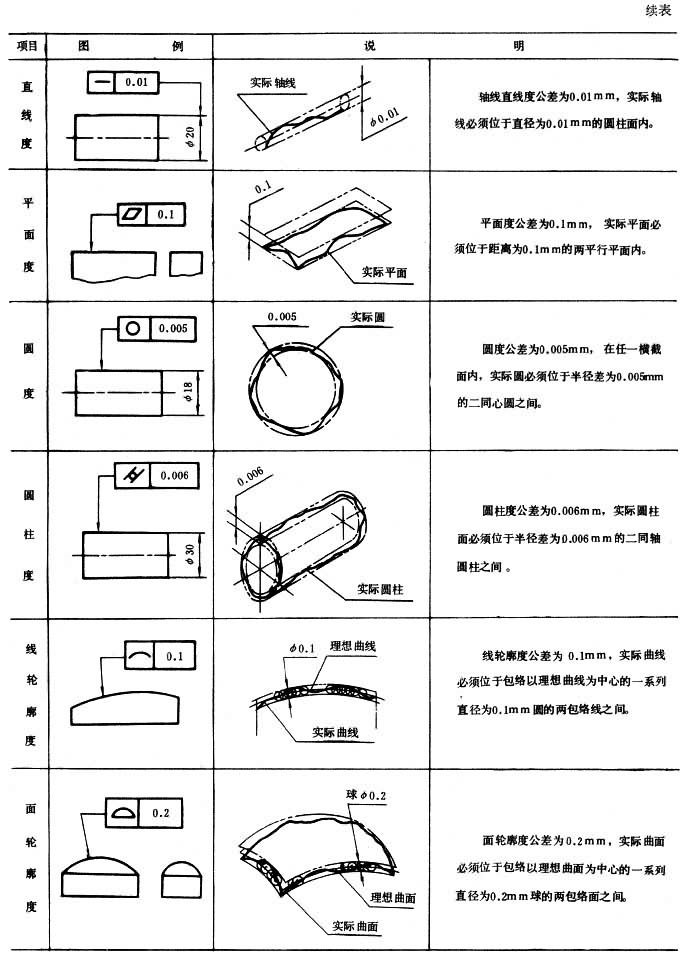
\includegraphics[width=0.9\linewidth]{data/image/13-1}
	\caption{}
%	\label{fig:13-1}
\end{figure}

\begin{figure}[h]
	\centering
	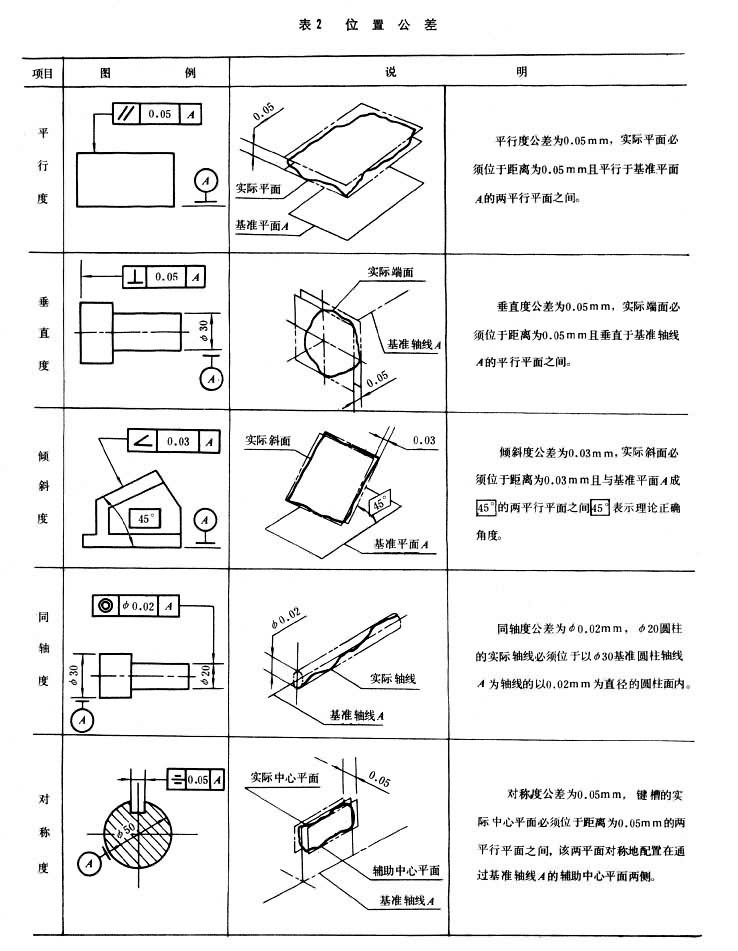
\includegraphics[width=0.9\linewidth]{data/image/13-2}
	\caption{}
%	\label{fig:13-2}
\end{figure}

\begin{figure}[h]
	\centering
	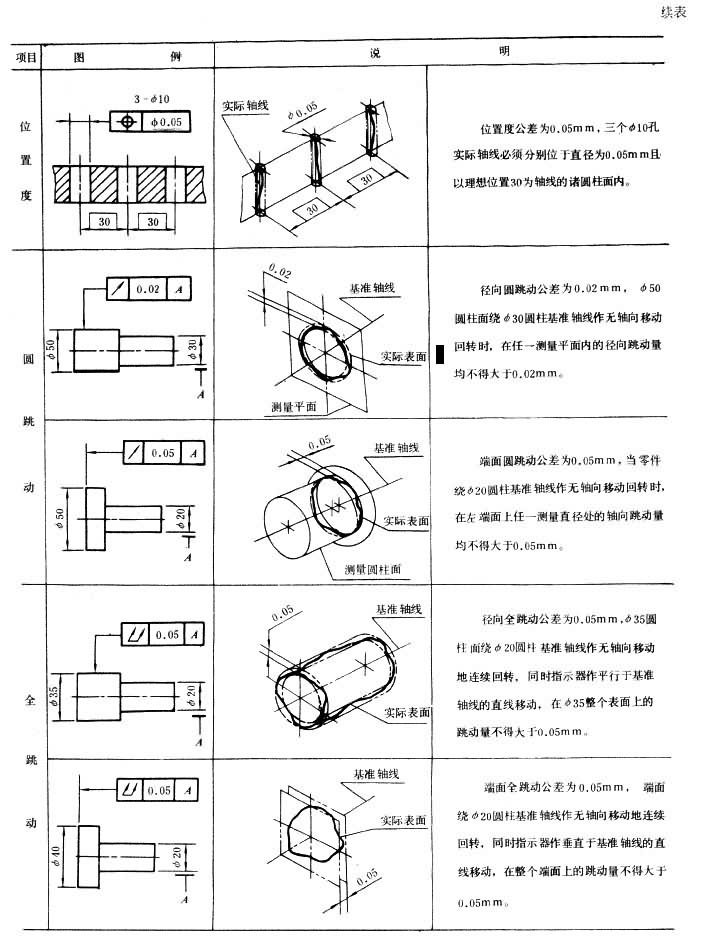
\includegraphics[width=0.9\linewidth]{data/image/13-3}
	\caption{}
%	\label{fig:13-3}
\end{figure}

\subsection{课堂小结}
\begin{enumerate}[1、]
	\item 平面的加工工工艺;
	\item 斜面的加工工艺;
	\item 形位公差;
	\item 编程实例。
\end{enumerate}

\vfill
\subsection{布置作业}
\begin{enumerate}[1、]
	\item 编写斜面的程序。
\end{enumerate}
\vfill